\documentclass[a4paper,12pt]{article}
\usepackage{amsmath,amssymb}
\usepackage[T2A]{fontenc}
\usepackage[russian]{babel}
\usepackage[utf8]{inputenc}
\usepackage{geometry}
\usepackage{listings}
\usepackage{xcolor}
\usepackage{float}
\usepackage{graphicx}
\usepackage{booktabs}
\usepackage{amsopn}
\usepackage{array}
\usepackage{multirow}
\usepackage{caption}
\geometry{margin=2cm, top=2cm, bottom=2cm}

% ── листинг в стиле IntelliJ ──────────────────────────────────────────
\definecolor{intj-bg}{HTML}{2B2B2B}
\definecolor{intj-key}{HTML}{CC7832}
\definecolor{intj-str}{HTML}{6A8759}
\definecolor{intj-comm}{HTML}{808080}
\definecolor{intj-id}{HTML}{A9B7C6}

\lstdefinestyle{intellij}{
  language=Python,
  backgroundcolor=\color{intj-bg},
  basicstyle=\ttfamily\footnotesize\color{intj-id},
  keywordstyle=\color{intj-key}\bfseries,
  stringstyle=\color{intj-str},
  commentstyle=\itshape\color{intj-comm},
  numberstyle=\color{intj-comm}\tiny,
  numbers=left,
  stepnumber=1,
  frame=single,
  rulecolor=\color{intj-comm},
  showstringspaces=false,
  breaklines=true,
  tabsize=4,
  xleftmargin=1.5em
}

% ─────────────────────────────────────────────────────────────────────
\begin{document}

% ══ ТИТУЛЬНЫЙ ЛИСТ ════════════════════════════════════════════════════
\begin{figure}[h]
    \centering
    \begin{minipage}{0.45\linewidth}
        \centering
        
\includegraphics[width=\linewidth]{slogan_chernyy}
    \end{minipage}
    \hfill
    \begin{minipage}{0.45\linewidth}
        \centering
        
\includegraphics[width=\linewidth]{cs-logo}
    \end{minipage}
\end{figure}

\begin{table}[htbp]
    \centering
    \begin{tabular}{lrlr}
        Группа        & \qquad\qquad P3219        & К работе допущен  & \qquad\qquad\qquad\qquad\qquad\qquad \\
        \cmidrule{2-2}\cmidrule{4-4}
        Студент       & \qquad\qquad Ануфриев А.С. & Работа выполнена  & \qquad\qquad\qquad\qquad\qquad\qquad \\
        \cmidrule{2-2}\cmidrule{4-4}
        Преподаватель & \qquad\qquad Зинченко А.А. & Отчёт принят      & \qquad\qquad\qquad\qquad\qquad\qquad \\
        \cmidrule{2-2}\cmidrule{4-4}
    \end{tabular}
\end{table}

\vspace{1.5cm}
\begin{center}
    \LARGE
    Вычислительная математика \\[8pt]
    Отчёт по лабораторной работе № 6 \\[6pt]
    Вариант 2
\end{center}

\vspace{9cm}
\begin{center}
    2026 год \\ Санкт-Петербург
\end{center}

\newpage
\tableofcontents

\newpage

% ══ РАЗДЕЛ 1 ══════════════════════════════════════════════════════════
\section{Цель работы}

Целью лабораторной работы является изучение и программная реализация численных методов
решения обыкновенных дифференциальных уравнений (ОДУ) первого порядка.
В соответствии с \textbf{вариантом 2} реализуются следующие методы:

\begin{enumerate}
    \item \textbf{Усовершенствованный метод Эйлера} (метод Хойна, метод предиктор-корректор 2-го порядка);
    \item \textbf{Метод Рунге--Кутта 4-го порядка};
    \item \textbf{Метод Милна} (многошаговый метод прогноза и коррекции 4-го порядка).
\end{enumerate}

Для каждого метода производится сравнение численного решения с точным,
оценивается погрешность, строятся графики.

% ══ РАЗДЕЛ 2 ══════════════════════════════════════════════════════════
\section{Рабочие формулы используемых методов}

\subsection{Постановка задачи Коши}

Требуется найти функцию $y = y(x)$, удовлетворяющую дифференциальному уравнению
первого порядка
\begin{equation}
    y' = f(x, y)
\end{equation}
и начальному условию
\begin{equation}
    y(x_0) = y_0.
\end{equation}

Численное решение состоит в построении таблицы значений $\{x_i, y_i\}$ на равномерной
сетке $x_i = x_0 + ih$, $i = 0, 1, \ldots, n$, $h = \mathrm{const}$.

\subsection{Усовершенствованный метод Эйлера (метод Хойна)}

Метод является одношаговым явным методом 2-го порядка точности.
На каждом шаге выполняется два вычисления правой части:

\begin{equation}
    \tilde{k}_1 = h \cdot f(x_i,\; y_i),
\end{equation}
\begin{equation}
    \tilde{k}_2 = h \cdot f(x_i + h,\; y_i + \tilde{k}_1),
\end{equation}
\begin{equation}
    \boxed{y_{i+1} = y_i + \dfrac{1}{2}\bigl(\tilde{k}_1 + \tilde{k}_2\bigr)}.
\end{equation}

\noindent Порядок точности: $\delta_n = O(h^2)$.\\
Погрешность оценивается \textbf{правилом Рунге}:
\begin{equation}
    R = \frac{|y^h_n - y^{h/2}_n|}{2^p - 1}, \quad p = 2,
\end{equation}
где $y^h_n$ "--- решение с шагом $h$, $y^{h/2}_n$ "--- с шагом $h/2$ в конечной точке.

\subsection{Метод Рунге--Кутта 4-го порядка}

Широко распространённый одношаговый метод 4-го порядка точности.
На каждом шаге выполняется четыре вычисления правой части:

\begin{align}
    k_1 &= h \cdot f(x_i,\; y_i), \\
    k_2 &= h \cdot f\!\left(x_i + \tfrac{h}{2},\; y_i + \tfrac{k_1}{2}\right), \\
    k_3 &= h \cdot f\!\left(x_i + \tfrac{h}{2},\; y_i + \tfrac{k_2}{2}\right), \\
    k_4 &= h \cdot f(x_i + h,\; y_i + k_3),
\end{align}
\begin{equation}
    \boxed{y_{i+1} = y_i + \frac{1}{6}(k_1 + 2k_2 + 2k_3 + k_4)}.
\end{equation}

\noindent Порядок точности: $\delta_n = O(h^4)$.\\
Погрешность оценивается правилом Рунге с $p = 4$.

\subsection{Метод Милна}

Метод Милна "--- многошаговый метод прогноза и коррекции 4-го порядка.
Для начала счёта необходимы значения в первых четырёх узлах
$y_0, y_1, y_2, y_3$, которые вычисляются методом Рунге--Кутта 4-го порядка.

\textbf{Этап прогноза} (явная формула):
\begin{equation}
    \boxed{y_i^{\text{прогн}} = y_{i-4} + \frac{4h}{3}\left(2f_{i-3} - f_{i-2} + 2f_{i-1}\right)},
    \quad f_j = f(x_j, y_j).
\end{equation}

\textbf{Этап коррекции} (неявная формула с итерациями):
\begin{equation}
    \boxed{y_i^{\text{корр}} = y_{i-2} + \frac{h}{3}\left(f_{i-2} + 4f_{i-1} + f_i^{\text{прогн}}\right)}.
\end{equation}

Коррекция повторяется до выполнения условия $|y_i^{(s+1)} - y_i^{(s)}| < \varepsilon_{\text{итер}}$.

\noindent Порядок точности: $\delta_n = O(h^4)$.\\
Погрешность многошагового метода оценивается как
\begin{equation}
    \varepsilon = \max_{0 \le i \le n} |y_i^{\text{точн}} - y_i|.
\end{equation}

% ══ РАЗДЕЛ 3 ══════════════════════════════════════════════════════════
\section{Вычислительная часть}

\subsection{Тестовый пример}

Рассмотрим уравнение
\[
    y' = y - x^2 + 1, \quad y(0) = 0{,}5, \quad x \in [0,\; 2], \quad h = 0{,}2.
\]
Точное решение: $y(x) = (x+1)^2 + Ce^x$, где $C = (y_0 - (x_0+1)^2)\,e^{-x_0} = -0{,}5$.

\begin{table}[H]
\centering
\caption{Численное решение тестового примера: $y' = y - x^2 + 1$}
\small
\begin{tabular}{r|r|rr|rr|rr}
\toprule
$i$ & $x_i$ &
\multicolumn{2}{c|}{Эйлер улучш.} &
\multicolumn{2}{c|}{Рунге--Кутта 4} &
\multicolumn{2}{c}{Милна} \\
 & & $y_i$ & $|\delta_i|$ & $y_i$ & $|\delta_i|$ & $y_i$ & $|\delta_i|$ \\
\midrule
0 & 0,0 & 0,50000000 & 0          & 0,50000000 & 0          & 0,50000000 & 0          \\
1 & 0,2 & 0,82600000 & 3,30e-3    & 0,82929333 & 5,29e-6    & 0,82929333 & 5,29e-6    \\
2 & 0,4 & 1,20692000 & 7,17e-3    & 1,21407621 & 1,14e-5    & 1,21407621 & 1,14e-5    \\
3 & 0,6 & 1,63724240 & 1,17e-2    & 1,64892202 & 1,86e-5    & 1,64892202 & 1,86e-5    \\
4 & 0,8 & 2,11023573 & 1,70e-2    & 2,12720268 & 2,69e-5    & 2,12720767 & 2,19e-5    \\
5 & 1,0 & 2,61768759 & 2,32e-2    & 2,64082269 & 3,64e-5    & 2,64082735 & 3,17e-5    \\
6 & 1,2 & 3,14957886 & 3,04e-2    & 3,17989417 & 4,74e-5    & 3,17990230 & 3,92e-5    \\
7 & 1,4 & 3,69368621 & 3,87e-2    & 3,73234007 & 5,99e-5    & 3,73234621 & 5,38e-5    \\
8 & 1,6 & 4,23509717 & 4,84e-2    & 4,28340950 & 7,43e-5    & 4,28341583 & 6,80e-5    \\
9 & 1,8 & 4,75561855 & 5,96e-2    & 4,81508569 & 9,06e-5    & 4,81508590 & 9,04e-5    \\
10& 2,0 & 5,23305463 & 7,24e-2    & 5,30536300 & 1,09e-4    & 5,30535692 & 1,15e-4    \\
\bottomrule
\end{tabular}
\end{table}

\subsection{Оценка погрешности}

\begin{table}[H]
\centering
\caption{Правило Рунге и max-погрешность для тестового примера ($h=0{,}2$)}
\begin{tabular}{lccc}
\toprule
Метод & Порядок $p$ & Рунге $R$ & $\varepsilon = \max|\delta_i|$ \\
\midrule
Эйлер усовершенствованный & 2 & $1{,}78 \cdot 10^{-2}$ & $7{,}24 \cdot 10^{-2}$ \\
Рунге--Кутта 4              & 4 & $6{,}80 \cdot 10^{-6}$ & $1{,}09 \cdot 10^{-4}$ \\
Милна                         & 4 & ---                    & $1{,}15 \cdot 10^{-4}$ \\
\bottomrule
\end{tabular}
\end{table}

\subsection{Сходимость при уменьшении шага}

\begin{table}[H]
\centering
\caption{Погрешности при различных шагах ($y' = 2y/x$, $y(1)=1$, $x \in [1,3]$)}
\begin{tabular}{crrr}
\toprule
$h$ & Эйлер улучш. $R$ & РК-4 $R$ & Милна $\varepsilon$ \\
\midrule
0,400 & $1,14 \cdot 10^{-1}$ & $6,89 \cdot 10^{-4}$ & $8,73 \cdot 10^{-3}$ \\
0,200 & $3,08 \cdot 10^{-2}$ & $4,24 \cdot 10^{-5}$ & $5,39 \cdot 10^{-4}$ \\
0,100 & $8,79 \cdot 10^{-3}$ & $3,05 \cdot 10^{-6}$ & $2,85 \cdot 10^{-5}$ \\
0,050 & $2,34 \cdot 10^{-3}$ & $2,04 \cdot 10^{-7}$ & $1,22 \cdot 10^{-6}$ \\
\bottomrule
\end{tabular}
\end{table}

При уменьшении $h$ вдвое погрешность уменьшается примерно в $4$ раза для метода
Эйлера (порядок~2) и примерно в $16$ раз для РК-4 и метода Милна (порядок~4),
что подтверждает теоретические оценки.

% ══ РАЗДЕЛ 4 ══════════════════════════════════════════════════════════
\section{Программная реализация}

\subsection{Описание программы}

Программа написана на языке \textbf{Python\,3} в виде одного консольного файла
\texttt{lab6.py}. Архитектура:

\begin{itemize}
    \item Каждый метод реализован в виде отдельной функции, возвращающей списки $\{x_i\}$, $\{y_i\}$.
    \item Уравнения хранятся в словаре; пользователь выбирает уравнение из предложенного списка (не менее трёх).
    \item Все вычисления выполнены \textbf{без} использования готовых численных библиотек (\texttt{scipy}, \texttt{odeint} и т.\,д.).
    \item Ввод с клавиатуры защищён от некорректных данных.
    \item Графики строятся с помощью \texttt{matplotlib} и сохраняются в файлы.
\end{itemize}

Главное меню предоставляет четыре режима:
\begin{enumerate}
    \item Интерактивное решение задачи Коши (выбор уравнения, ввод $x_0, y_0, x_n, h, \varepsilon$);
    \item Демонстрационный пример с фиксированными параметрами;
    \item Автоматический тест: три уравнения $\times$ три шага, проверка сходимости;
    \item Справка по формулам методов.
\end{enumerate}

\subsection{Листинг программы}

\subsubsection{Методы решения ОДУ}

\begin{lstlisting}[style=intellij, caption={Усовершенствованный метод Эйлера (метод Хойна)}]
def euler_improved(f, x0, y0, xn, h):
    """Improved Euler method (Heun's method / Euler with correction)."""
    xs, ys = [x0], [y0]
    x, y = x0, y0
    steps = round((xn - x0) / h)
    for _ in range(steps):
        k1 = h * f(x, y)
        k2 = h * f(x + h, y + k1)
        y = y + 0.5 * (k1 + k2)
        x = round(x + h, 10)
        xs.append(x); ys.append(y)
    return xs, ys
\end{lstlisting}

\begin{lstlisting}[style=intellij, caption={Метод Рунге--Кутта 4-го порядка}]
def runge_kutta4(f, x0, y0, xn, h):
    """Fourth-order Runge-Kutta method."""
    xs, ys = [x0], [y0]
    x, y = x0, y0
    steps = round((xn - x0) / h)
    for _ in range(steps):
        k1 = h * f(x,         y)
        k2 = h * f(x + h/2,   y + k1/2)
        k3 = h * f(x + h/2,   y + k2/2)
        k4 = h * f(x + h,     y + k3)
        y = y + (k1 + 2*k2 + 2*k3 + k4) / 6
        x = round(x + h, 10)
        xs.append(x); ys.append(y)
    return xs, ys
\end{lstlisting}

\begin{lstlisting}[style=intellij, caption={Метод Милна (прогноз-коррекция)}]
def milne(f, x0, y0, xn, h):
    """
    Milne's predictor-corrector method (4th order).
    The first 4 points (indices 0..3) are computed by RK4.
    Prediction: y[i] = y[i-4] + 4h/3*(2f[i-3] - f[i-2] + 2f[i-1])
    Correction: y[i] = y[i-2] + h/3*(f[i-2] + 4f[i-1] + f_pred)
    """
    steps = round((xn - x0) / h)
    if steps < 4:
        raise ValueError("Milne method requires at least 4 steps")

    # Bootstrap: first 4 points via RK4
    xs_init, ys_init = runge_kutta4(f, x0, y0, round(x0 + 3*h, 10), h)
    xs = list(xs_init)
    ys = list(ys_init)
    fs = [f(xs[i], ys[i]) for i in range(4)]

    for i in range(4, steps + 1):
        y_pred = ys[i-4] + (4*h/3) * (2*fs[i-3] - fs[i-2] + 2*fs[i-1])
        x_new  = round(x0 + i*h, 10)
        f_pred = f(x_new, y_pred)

        # Iterative correction until convergence
        y_corr = ys[i-2] + (h/3) * (fs[i-2] + 4*fs[i-1] + f_pred)
        for _ in range(50):
            f_corr = f(x_new, y_corr)
            y_new  = ys[i-2] + (h/3) * (fs[i-2] + 4*fs[i-1] + f_corr)
            if abs(y_new - y_corr) < 1e-12:
                y_corr = y_new
                break
            y_corr = y_new

        xs.append(x_new)
        ys.append(y_corr)
        fs.append(f(x_new, y_corr))
    return xs, ys
\end{lstlisting}

\subsubsection{Оценка погрешности}

\begin{lstlisting}[style=intellij, caption={Правило Рунге и max-погрешность}]
def runge_error(method, f, x0, y0, xn, h, p):
    """Runge rule at the interval end."""
    _, yh  = method(f, x0, y0, xn, h)
    _, yh2 = method(f, x0, y0, xn, h/2)
    R = abs(yh[-1] - yh2[-1]) / (2**p - 1)
    return R

def exact_error(f_exact, xs, ys, C):
    """eps = max|y_exact - y_numerical|"""
    errs = [abs(f_exact(x, C) - y) for x, y in zip(xs, ys)]
    return max(errs)
\end{lstlisting}

\subsection{Скриншоты результатов}

\subsubsection{Пример 1: $y' = y - x^2 + 1$, $y(0)=0{,}5$, $h=0{,}2$}

\begin{figure}[H]
    \centering
    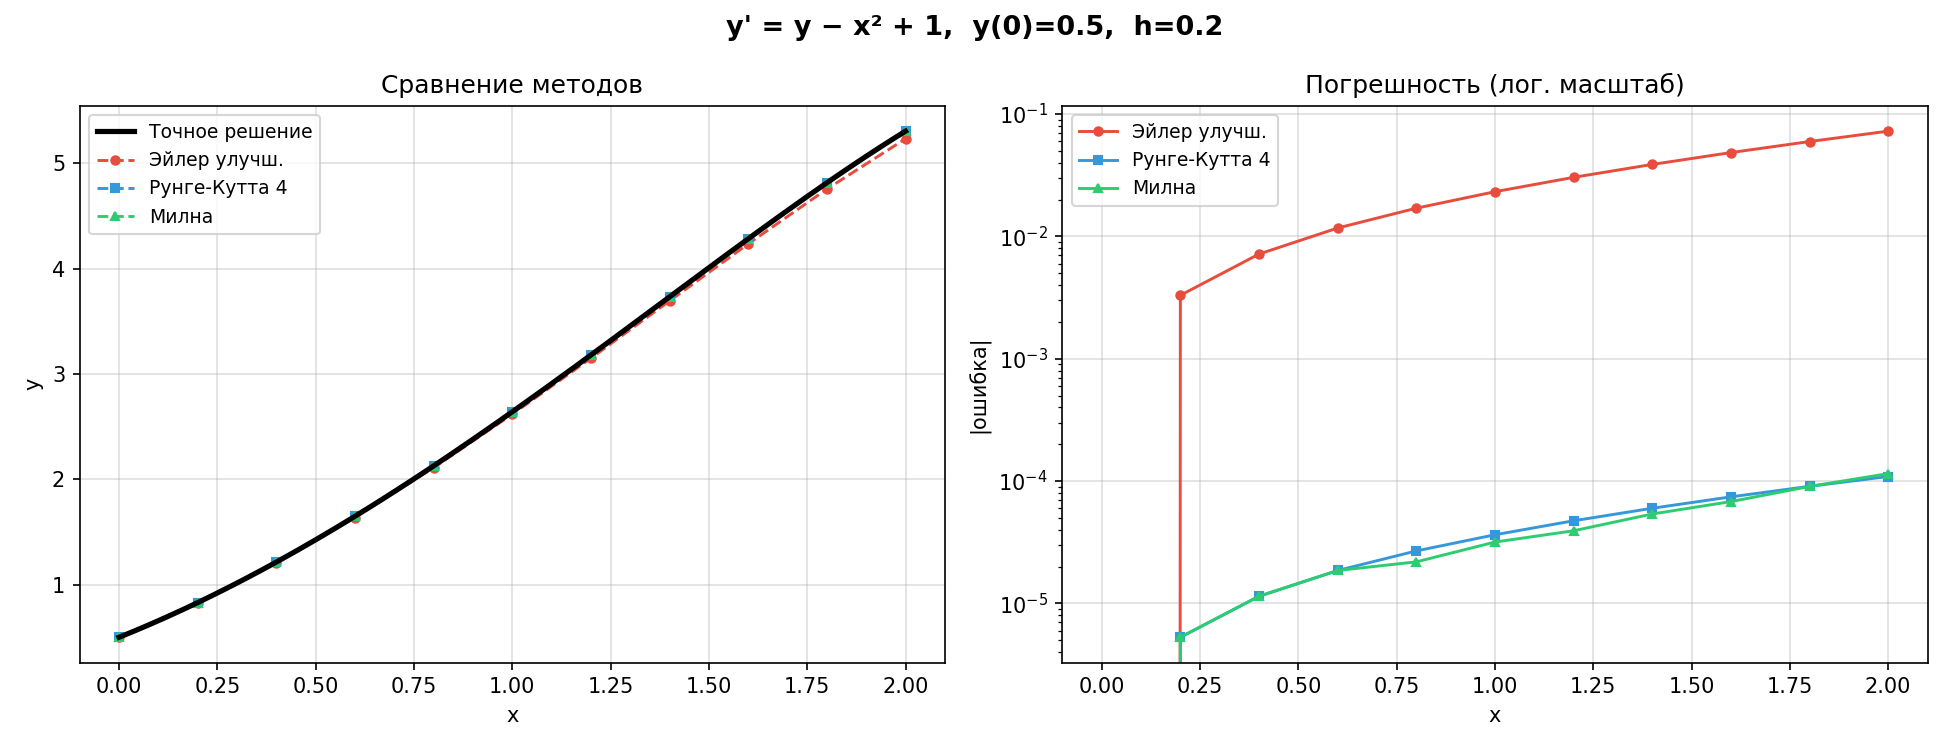
\includegraphics[width=\linewidth]{scr1}
    \caption{Сравнение методов и погрешности для уравнения $y' = y - x^2 + 1$}
\end{figure}

\subsubsection{Пример 2: $y' = x + y$, $y(0)=1$, $h=0{,}1$}

\begin{figure}[H]
    \centering
    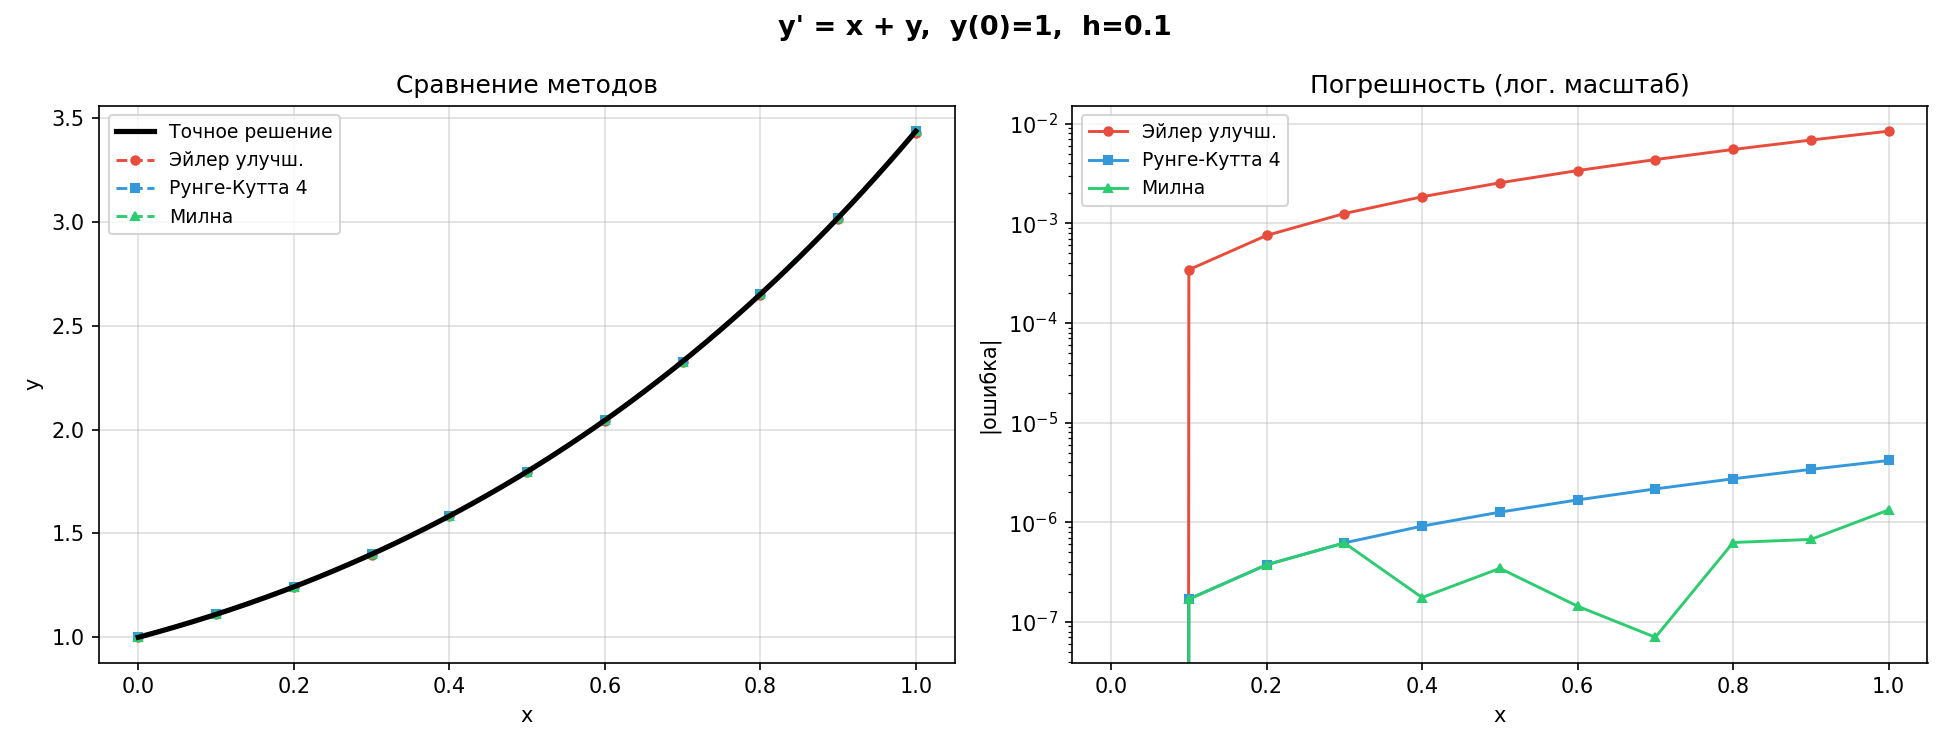
\includegraphics[width=\linewidth]{scr2}
    \caption{Сравнение методов и погрешности для уравнения $y' = x + y$}
\end{figure}

\subsubsection{Пример 3: Сходимость при уменьшении шага ($y' = 2y/x$)}

\begin{figure}[H]
    \centering
    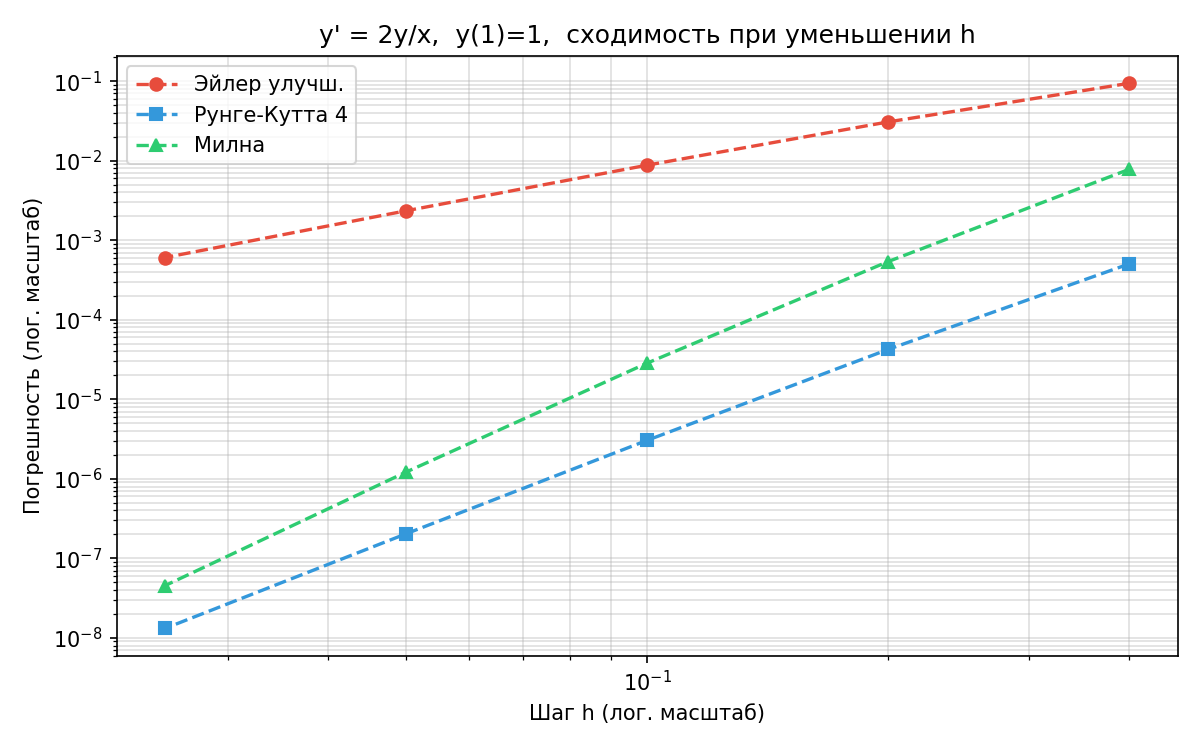
\includegraphics[width=0.7\linewidth]{scr3}
    \caption{Зависимость погрешности от шага $h$ (лог-лог масштаб)}
\end{figure}

% ══ РАЗДЕЛ 5 ══════════════════════════════════════════════════════════
\section{Выводы}

В ходе выполнения лабораторной работы были исследованы три численных метода
решения задачи Коши для ОДУ первого порядка.

\begin{enumerate}
    \item \textbf{Усовершенствованный метод Эйлера} (порядок~2) прост в реализации и
    требует двух вычислений правой части на каждом шаге. Погрешность убывает как $O(h^2)$,
    что подтверждается правилом Рунге: при уменьшении $h$ вдвое погрешность
    уменьшается примерно в~4 раза.

    \item \textbf{Метод Рунге--Кутта 4-го порядка} (порядок~4) существенно точнее:
    при тех же шагах погрешность на 3--4 порядка ниже. Требует четырёх вычислений
    правой части за шаг, но это оправдано высокой точностью. Правило Рунге
    подтверждает уменьшение погрешности в~16 раз при делении шага вдвое.

    \item \textbf{Метод Милна} (порядок~4) демонстрирует точность, сопоставимую с
    РК-4, при меньшем числе вычислений правой части в основном цикле
    (одно вычисление вместо четырёх), однако требует стартовых значений,
    получаемых методом РК-4. Ограничение: необходимо не менее 4 шагов на интервале.

    \item При уменьшении шага все методы демонстрируют теоретически
    ожидаемую скорость сходимости, что подтверждает корректность реализации.

    \item Программа устойчива к некорректным входным данным: реализована
    валидация ввода, и при недостаточном числе шагов для метода Милна
    генерируется информативное исключение.
\end{enumerate}

\end{document}
